\documentclass[12pt]{article}

%-------------PACKAGES------------- 
\usepackage[margin=1in]{geometry} 
\usepackage{amsmath,amsthm,amssymb}
\usepackage{pgfplots}
\usepackage{float}
\usepackage{braket}
\usepackage{titling}
\usepackage{tikz}
\usepackage{mathtools}
\usepackage{listings}
\usepackage{color}
\usepackage{caption}
\usepackage{subcaption}
\usepackage{algorithm,algpseudocode}

%-------------FORMATTING-------------
\setlength{\droptitle}{-6em} 
\setlength{\parindent}{0pt}
 
%--------------COMMANDS--------------
\newcommand{\N}{\mathbb{N}}
\newcommand{\Z}{\mathbb{Z}}
\newcommand{\R}{\mathbb{R}}
\newcommand{\C}{\mathbb{C}}
%\renewcommand{\qedsymbol}{\filledbox}

\DeclarePairedDelimiter \abs{\lvert}{\rvert}%
\DeclarePairedDelimiter \babs{\bigg\lvert}{\bigg\rvert}%
\DeclarePairedDelimiter \norm{\lVert}{\rVert}%

%------------ENVIRONMENTS------------- 
\newenvironment{theorem}[2][]{\begin{trivlist}
\item[{\bfseries #1}\hskip \labelsep {\bfseries #2.}]}{\end{trivlist}}
\newenvironment{lemma}[2][Lemma]{\begin{trivlist}
\item[\hskip \labelsep {\bfseries #1}\hskip \labelsep {\bfseries #2.}]}{\end{trivlist}}
\newenvironment{exercise}[2][Exercise]{\begin{trivlist}
\item[\hskip \labelsep {\bfseries #1}\hskip \labelsep {\bfseries #2.}]}{\end{trivlist}}
\newenvironment{reflection}[2][Reflection]{\begin{trivlist}
\item[\hskip \labelsep {\bfseries #1}\hskip \labelsep {\bfseries #2.}]}{\end{trivlist}}
\newenvironment{proposition}[2][Proposition]{\begin{trivlist}
\item[\hskip \labelsep {\bfseries #1}\hskip \labelsep {\bfseries #2.}]}{\end{trivlist}}
\newenvironment{corollary}[2][Corollary]{\begin{trivlist}
\item[\hskip \labelsep {\bfseries #1}\hskip \labelsep {\bfseries #2.}]}{\end{trivlist}}
\theoremstyle{remark}
\newtheorem*{remark}{Remark}

%-------------CODE-STYLE------------
\definecolor{dkgreen}{rgb}{0,0.6,0}
\definecolor{gray}{rgb}{0.5,0.5,0.5}
\definecolor{mauve}{rgb}{0.58,0,0.82}
\lstset{frame=tb,
	language=C++,
	aboveskip=3mm,
	belowskip=3mm,
	showstringspaces=false,
	columns=flexible,
	basicstyle={\small\ttfamily},
	numbers=none,
	numberstyle=\tiny\color{gray},
	keywordstyle=\color{blue},
	commentstyle=\color{dkgreen},
	stringstyle=\color{mauve},
	breaklines=true,
	breakatwhitespace=true,
	tabsize=3
}

\lstset{
	morekeywords={end}
}

%------------------------------------ 
%---------START-OF-DOCUMENT----------
%------------------------------------

\begin{document}
 
\title{Homework 11}
\author{David Miller \\ 
MAP5345: Partial Differential Equations I} 
 
\maketitle

\section*{Problem 1}

\textit{Consider polar coordinates $(r,\theta)$, whic are related to Cartesian coordinates via $x = rcos\theta$ and $y = rsin\theta$.} \\

\textit{a) Use the chain rule for partial derivatives to calculate $\frac{\partial}{\partial r}, \frac{\partial^2}{\partial r^2}, \frac{\partial}{\partial\theta}, \frac{\partial^2}{\partial\theta^2}$ in terms of x and y partial derivatives.} \\

The coordinate transformation
\begin{align*}
	x \mapsto r\cos(\theta), \quad y \mapsto r\sin(\theta)
\end{align*}
yields the following
\begin{align*}
u_\theta & = u_xx_\theta + u_yy_\theta = -u_xr\sin(\theta) + u_yr\cos(\theta)
\\ \\
u_r & = u_xx_r + u_yy_r = -u_x\sin(\theta) + u_y\cos(\theta)
\\ \\
u_{\theta\theta} & = -r\cos(\theta)u_x - r\sin(\theta)\partial_\theta u_x - r\sin(\theta)u_y + r\cos(\theta)\partial_\theta u_y \\
& = -r\cos(\theta)u_x - r\sin(\theta)\bigg(-u_{xx}r\sin(\theta) + u_{xy}r\cos(\theta)\bigg) \\ & - r\sin(\theta)u_y + r\cos(\theta)\bigg(-ru_{xy}\sin(\theta) + u_{yy}r\cos(\theta)\bigg) \\ 
& = -r\bigg(\cos(\theta)u_x + \sin(\theta)u_y\bigg) + r^2\bigg(\sin^2(\theta)u_{xx} -2\cos(\theta)\sin(\theta)u_{xy} + \cos^2(\theta)u_{yy}\bigg) 
\\ \\
u_{rr} & = \cos(\theta)\partial_ru_x + \sin(\theta)\partial_ru_y \\
& = \cos^2(\theta)u_{xx} + 2\cos(\theta)\sin(\theta)u_{xy} + \sin^2(\theta)u_{yy}
\end{align*}

\newpage

\textit{b) Use your results to show that the Laplacian in polar coordiantes is given by}
\begin{align*}
	\Delta u = u_{rr} + \frac{1}{r}u_r + \frac{1}{r^2}u_{\theta\theta}
\end{align*}

Dividing the expression for $u_{\theta\theta}$ yields
\begin{align*}
	\frac{1}{r^2}u_{\theta\theta} = -\frac{1}{r}u_r + \sin^2(\theta) u_{xx} - 2\cos(\theta)\sin(\theta)u_{xy} + \cos^2(\theta)u_{yy}
\end{align*}
Then adding the above to $u_{rr}$ gets us
\begin{align*}
	& u_{rr} + \frac{1}{r^2}u_{\theta\theta} = -\frac{1}{r}u_r + u_{xx} + u_{yy} \\
	\Rightarrow \quad & u_{xx} + u_{yy} = u_{rr} + \frac{1}{r}u_r + \frac{1}{r^2}u_{\theta\theta}
\end{align*}

\newpage

\section*{Problem 2}

\textit{Using Julia, graph $J_0(x)$, i.e. the Bessel function of the first kind and of order n = 0. Choose a reasonable domain to graph the function, so that you can see at least a few roots of $J_0$. On the same graph, plot the function}
\begin{align}
	\sqrt{\frac{2}{\pi x}}\cos(x - \pi/4 -n\pi/2)
\end{align} 
\textit{and verify that the two are asymptotic for $x >> 1$. How many roots do you have to go out for the asymptotic formula to capture the roots pretty accurately? Do the same for $J_1(x)$, the first-kind Bessel function of order $n = 1$. Also, verify the asymptotic formula.}

\begin{figure}[H]
	\centering
	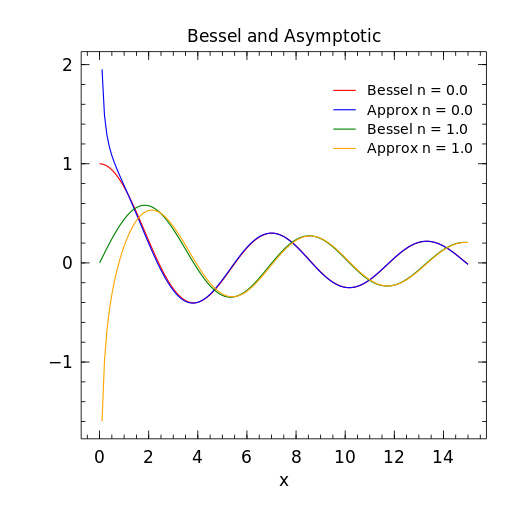
\includegraphics[width=13cm]{HW11.png}
	\caption{Bessel Function plotted against its asymptotic formula.}
\end{figure}

\newpage

\section*{Problem 3}

\textit{For a drum head with given wave-speed c and radius a, can you determine the fundamental frequency, and thus the 'pitch' of the sound that drum will produce? For a realistic drum with c = 400 m/s and a = 0.5, what is the fundamental frequency in Hz? Also find the first harmonic.} \\

The fundamental frequency will be the first root of $J_0$, the 	$0-th$ order Bessel function, times the wave speed $c$. Similarly the $n-th$ harmonic will be the $n+1-th$ root of $J_0$. From this we get
\begin{center}
	\begin{tabular}{|c|c|}
		\hline
		\textbf{Harmonic} & \textbf{Frequency (Hz)} \\ \hline \hline
		0 (Fundamental) & 1923.8608 \\ \hline
		1 & 4416.0624 \\ \hline
		2 & 6922.9816 \\ \hline
		3 & 9433.2272 \\ \hline
		4 & 11944.7336 \\ \hline
		\vdots & \vdots \\ \hline
	\end{tabular}
\end{center}

\newpage

\section*{Problem 4}

\textit{Consider the Bessel ODE derived in class. Put this ODE into the form of a Sturm-Liouville problem. What is the weighted inner product for which the functions $R_m(r) = J_0(\sqrt{\lambda}r)$ are orthogonal?} \\

The Sturm-Liouville equation
\begin{align*}
	(p(x)u^\prime(x))^\prime - q(x)u(x) = -\lambda m(x)u(x)
\end{align*} 
has inner product (orthogonal functions)
\begin{align*}
	\braket{f,g} = \int m(x)f(x)\overline	{g(x)} \, dx
\end{align*}
The ODE we have in class can be multiplied by $r$ to obtain
\begin{align*}
	R^{\prime\prime}(r) + \frac{1}{r}R^{\prime}(r) + R(r)\bigg(\lambda - \frac{n^2}{r^2}\bigg) = 0 \\
	rR^{\prime\prime}(r) + R^{\prime}(r) + rR(r)\bigg(\lambda - \frac{n^2}{r^2}\bigg) = 0 \tag{multiply by $r$} \\
	\Rightarrow \quad u = R(r), \quad p = r, \quad q = \frac{n^2}{r}, \quad m = r
\end{align*}
Therefore $r$ is the weight that makes the Bessel functions orthogonal. The resulting inner product for the Bessel functions is 
\begin{align*}
	\braket{R_i, R_j} = 2\pi\int rR_iR_j \, dr
\end{align*}
where the $2\pi$ comes from the integral about the $\theta$ domain $[0,2\pi]$.

\newpage

\section*{Problem 5}

\textit{Consider radial vibrations of a circular drum of radius a = 0.5 m. The medium's speed of sound given by c = 400 m/s.} \\

\textit{a) Now, suppose that the initial displacement is $u_0 = a^2 - r^2$ and there is no initial velocity. Write don the exact solution to the IBVP.} \\

The general solution of the PDE under rotational invariance is 
\begin{align*}
u(r,t) = \sum\limits_{n=1}^\infty (A_n\cos(\sqrt{\lambda_n}ct) + B_n\sin(\sqrt{\lambda}ct))J_0(\sqrt{\lambda_n}r)
\end{align*}
but under zero initial velocity we get $B_n = 0$ and are left with
\begin{align*}
u(r,t) = \sum\limits_{n=1}^\infty A_n\cos(\sqrt{\lambda_n}ct)J_0(\sqrt{\lambda_n}r)
\end{align*}
Using projection to determine $A_n$ we arrive at 
\begin{align*}
A_n & = \frac{\braket{a^2 - r^2, J_0(\sqrt{\lambda_n}r)}}{\braket{J_0(\sqrt{\lambda_n}r),J_0(\sqrt{\lambda_n}r)}} = \frac{\int_0^{0.5}(a^2 - r^2)J_0(\sqrt{\lambda_n}r)r \, dr}{\int_0^{0.5}J_0(\sqrt{\lambda_n}r)J_0(\sqrt{\lambda_n}r)r \, dr}
\end{align*}
Therefore the exact solution is 
\begin{align*}
	\sum\limits_{n=1}^\infty A_n\cos(\sqrt{\lambda_n}ct)J_0(\sqrt{\lambda_n}r), \quad A_n = \frac{\int_0^{0.5}(a^2 - r^2)J_0(\sqrt{\lambda_n}r)r \, dr}{\int_0^{0.5}J_0(\sqrt{\lambda_n}r)J_0(\sqrt{\lambda_n}r)r \, dr}
\end{align*}

\textit{b) Perform the projection numerically, using the trapezoidal rule, in order to find a numerical approximation to the first three coefficients in your solution.} \\

Using the trapezoidal rule to perform quadrature we get the follwoing coefficients
\begin{align*}
	A_1 \approx  0.0375909, \quad A_2 \approx 0.0194997, \quad A_3 \approx −0.0047067
\end{align*}

\textit{c) Visualize a few different time-values of this approximate solution in Julia.}

\newpage

\section*{Decay Coefficients}

\textit{Find the lower bounds of the following functions} \\

\begin{theorem}{Theorem 1}
	If $f_{ext} \in C^n$ then there exists a $M$ such that $c_k \leq \frac{M}{\abs{k}^n}$
\end{theorem}

\begin{theorem}{Theorem 2}
	If $f_{ext} \in L^2$ and if $c_k = \frac{\braket{f, e^{ikx}}}{\braket{e^{ikx}, e^{ikx}}}$ and there exists $M$, $\epsilon > 0$ such that $\abs{c_k} \leq \frac{M}{\abs{k}^{1+n+\epsilon}}$ then $f_{ext} \in C^n$
\end{theorem}

\textit{a) $\abs{x}$} \\

We know that $f_{ext} \in C^0$ and therefore $f_{ext} \not\in C^1$ and the decay rate is bounded below by 0. From Theorem 2 we then know that $\not\exists M$ or $\epsilon$ such that $\abs{c_k} \leq \frac{M}{\abs{k}^{2+\epsilon}}$ and therefore the decay rate is bounded above by 2. \\

\textit{b) x} \\

We know that $f_{ext}$ is piecewise polynomial and therefor $f_{ext} \not\in C^0$ and the decay rate is bounded below by some constant $M$. From Theorem 2 we then know that $\not\exists M$ or $\epsilon$ such that $\abs{c_k} \leq \frac{M}{\abs{k}^{1+\epsilon}}$ and therefore is bounded above by 1. \\

\textit{c) $\pi^2 - x^2$} \\

Since $f_{ext} \in C^0$ the proof follows similarly from part (a). Therefore the decay rate is bounded below by 0 and above by 2. \\

\textit{d) $\sqrt{\pi^2 - x^2}$} \\ 

Since $f_{ext} \in C^0$ the proof follows similarly from part (a). Therefore the decay rate is bounded below by 0 and above by 2. \\

\textit{e) $x(\pi^2 - x^2)$} \\ 

We know that $f_{ext} \in C^1$ and therefore $f_{ext} \not\in C^2$ and the decay rate is bounded below by 1. From Theorem 2 we then know that $\not\exists M$ or $\epsilon$ such that $\abs{c_k} \leq \frac{M}{\abs{k}^{3+\epsilon}}$ and therefore the decay rate is bounded above by 3. \\

\textit{f) $(\pi^2 - x^2)^2$} \\

We know that $f_{ext} \in C^2$ and therefore $f_{ext} \not\in C^3$ and the decay rate is bounded below by 2. From Theorem 2 we then know that $\not\exists M$ or $\epsilon$ such that $\abs{c_k} \leq \frac{M}{\abs{k}^{4+\epsilon}}$ and therefore the decay rate is bounded above by 4. \\

\end{document}